\documentclass{article}

%----------------------------------------------------------------------------------------
%	PACKAGES AND OTHER DOCUMENT CONFIGURATIONS
\usepackage[utf8]{inputenc}
\usepackage{graphicx}
\usepackage{tabularx}
\usepackage[export]{adjustbox}
\usepackage{paralist}
\usepackage{wrapfig}
\usepackage{float}
\usepackage{geometry}
 \geometry{
 a4paper,
 total={170mm,257mm},
 left=20mm,
 top=20mm,
 }

%----------------------------------------------------------------------------------------
\newcommand*{\plogo}{\fbox{$\mathcal{PL}$}} % Generic publisher logo

%----------------------------------------------------------------------------------------
%	TITLE PAGE
%----------------------------------------------------------------------------------------

\newcommand*{\titleGP}{\begingroup % Create the command for including the title page in the document
\centering % Center all text
\vspace*{\baselineskip} % White space at the top of the page

\rule{\textwidth}{1.6pt}\vspace*{-\baselineskip}\vspace*{2pt} % Thick horizontal line
\rule{\textwidth}{0.4pt}\\[\baselineskip] % Thin horizontal line

{\LARGE Caracal Automated Marking \\ Software Requirements \\ Specification}\\[0.2\baselineskip]  % Title 

Version: (1.0.0) 


\rule{\textwidth}{0.4pt}\vspace*{-\baselineskip}\vspace{3.2pt} % Thin horizontal line
\rule{\textwidth}{1.6pt}\\[\baselineskip] % Thick horizontal line

\scshape % Small caps
\vspace*{2\baselineskip} % Whitespace between location/year and editors

Edited by \\[\baselineskip]
{\Large Oratile Motswagosele \\ Mankgwanyane Tlaka \\ Lesego Makaleng \\ Kenneth Mangwane \par} % Editor list

{\itshape University of Pretoria\par} % Editor affiliation

\begin{figure}[t]
\centering
	
\includegraphics[width=350px]{Images/UP_Logo}
\end{figure}

{\scshape 2017} \\[0.3\baselineskip] % Year published
{ Project Client: Caracal Research}\par % Publisher

\endgroup}

\begin{document}

\titleGP % This command includes the title page
\pagebreak

\clearpage
\tableofcontents
\clearpage

\section{Vision and Scope}
	\subsection{Project Background}
	E-learning is a topic that receives a lot of attention worldwide and even more in Africa. The problem of ed-
ucating dispersed people with few resources is a headache that troubles many government and new initiatives
are being launched daily to try and solve the problem. \\\\
Taking a deeper look at the grade 12 question paper marking process, it is realised that most of the time,
individuals are still needed who have the knowledge and skill to go through all the answered mathematics scripts
and grade them correctly. This process has proven to be time costly and human error tends to creep up at a
minimal level.

	\subsection{Project Vision}
	Caracal Automated Marking is aimed at developing a metalanguage for the electronic assessment of grade 12
mathematical question in which the steps employed to arrive at the answer can be assessed. Not only the final answer.
The system should be ideally available as a Moodle plugin. The proposed solution, 
ideally would be integrated into the Moodle open learning platform as a plugin. \\\\
The system should accept three documents, i.e. a document with mathematics question; a document with the
memorandum and a document with student answers. The system should analyze answer document and give a
mark.
At the end the proposed system should ideallly act as methodology through which any given problem and
matching memorandum can be entered.

	\subsection{Architecture Design}
		\subsubsection{Architectural Patterns}
		\subsubsection{Quality Requirements}
		\subsubsection{Architectural Tactics}
	
	\subsection{Project Scope}
	E-learning is a topic that is receiving a huge amount of attention worldwide and especially in South Africa.
Currently most e-learning in schools consists of taking paper material and making it available on electronic
devices such as tablets. \\\\
LMS systems such as Moodle gives the option to design and enter electronic courses and presenting assess-
ments in the form of multiple choice and other one-dimensional methods. The available commerical systems
are available but cost is a problem.

\section{Modularization}
	\subsection{Access Module}
		\subsubsection{Scope}
			 The scope of this module will be to give users a graphical user interface, which will allow them to login/register and also to be able to have access to the system as whole.Access to the entire system will be made possible by making use of a request and render process , see the domain below. This module will be in charge of deploying a GUI on multiple browsers i.e. FireFox, Google Chrome, Microsoft Edge. Web browser will be the only supported access channel  and recommended devices will be limited to a desktop or laptop only. 
		
			 \begin{figure}[H]
			\centering
				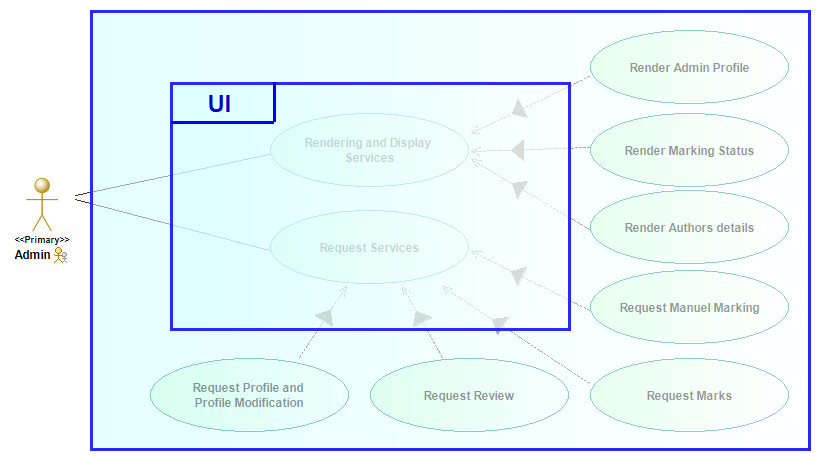
\includegraphics[width=450px]{Images/Access_Module/Pictures/Acess_Use_Case_Diagram_Scope}
			\end{figure}
		\subsubsection{Domain Model}
			\begin{figure}[H]
			\centering
				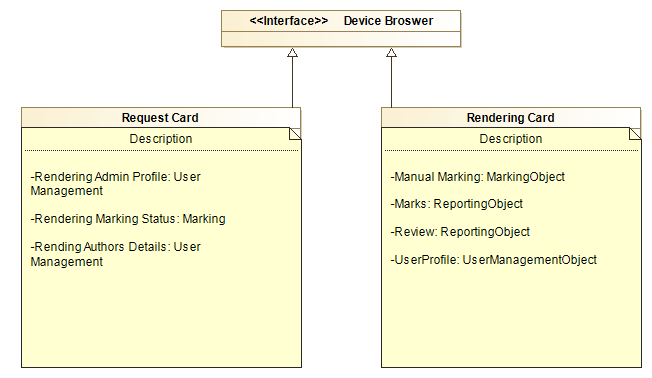
\includegraphics[width=450px]{Images/Access_Module/Pictures/Access_module_Class_diagram}
			\end{figure}
			
			\par The domain model above shows how the system will make use of a card system. where the user will be able 
			to interact with the entire system to the use of only interacting with one card at the time. The render 
			card will be be responsible to render and display all the functionality requested from the Request card.
		
			
		\subsubsection{Technologies}
			\paragraph{Programming Languages}
				\begin{enumerate}
 					 \item Python
 					 		Due to python's ability of being a general purpose language and both a scripting language
 					 		we will use it as a scripting language to connect to the server so that we will be able to
 					 		render requested functionality to the user.
  						\item PHP
  							\par PHP will be our main language for developing the website. mainly for its ability to be both 	
  							server side and client side, this will reduce number of different languages to be used.
  							
  							\par frameworks such as bootstrap will be used for the design of the 
  							layout of the user interface and human
  							computer interaction principles will be followed.
				\end{enumerate}
				
			\paragraph{Web Development Technologies}
				\paragraph{Symfony \newline}	
					 Symfony is a PHP web application framework and a set of reusable PHP components/libraries.
					Symfony aims to speed up the creation and maintenance of web applications and to 
					replace repetitive coding tasks.
					Symfony has a low performance overhead used with a bytecode cache.Symfony is aimed at building robust applications in an enterprise context, and aims to
					 give developers full control over the configuration: from the directory structure to the
					  foreign libraries, almost everything can be customized. To match enterprise
					   development guidelines, Symfony is bundled with additional tools to help developers test, debug 
					  and document project
					  
					  Symfony makes heavy use of existing PHP open-source projects as part of the framework, including:
					  \begin{itemize}
					  	\item Propel or Doctrine as object-relational mapping layers
					  	\item PDO database abstraction layer 
					  	\item PHPUnit, a unit testing framework
					  	\item Twig, a templating engine
					  	\item Swift Mailer, an e-mail library
					  \end{itemize}
					  
				

	\subsection{User Management Module}
		\subsubsection{Scope}
		This module will be in charge of managing user information and the different types of users. The different
		types of users of this system will be as follows:
			\begin{itemize}
				\item{Admin - The role of this user will be to have access to uploading question papers and memorandums,
					  	and general access to sensitive information of the system. This user can also delete/approve other
						users below this level i.e. Teachers from the system.}
				\item{Teacher - The role of this user will be to upload the test papers of students i.e. their class of students,
						and recieve marks of the papers they have uploaded. This user cannot have direct access to the memo
						or question paper. This user also needs approval from the admin before being registered. This is to prevent 
						students registering as fake teachers and uploading tests to get access to the marking system}
			\end{itemize}
			
			\begin{figure}[h]
				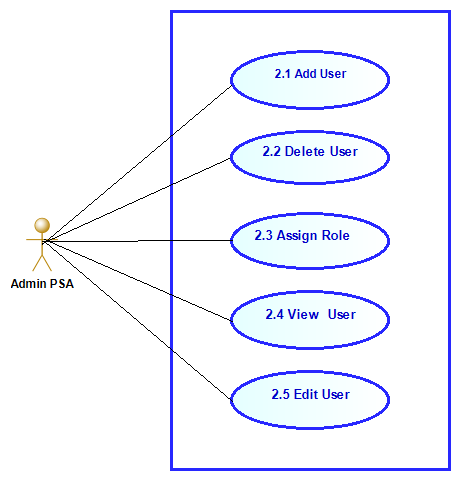
\includegraphics[scale=0.6]{Images/User_Management_Module/UserManagementModuleUseCase}
				\caption{User Management Module Use Case}
			\end{figure}
			
		\subsubsection{Domain Model}
						\begin{figure}[h]
					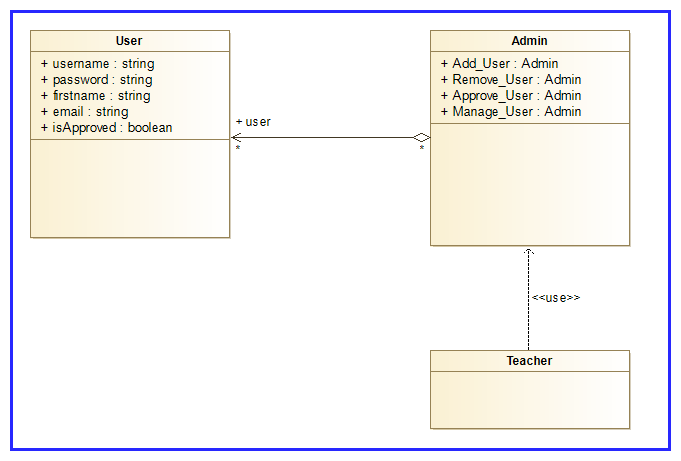
\includegraphics[scale=0.6]{Images/User_Management_Module/UserManagementModuleDomainModel}
					\caption{User Management Module Domain Model}
				\end{figure}
				
		\subsubsection{Service Contracts}
						\begin{figure}[h]
					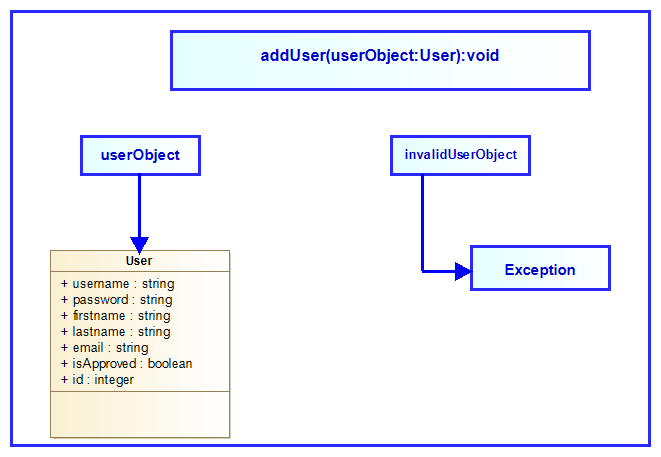
\includegraphics[scale=0.6]{Images/User_Management_Module/UserManagementModuleServiceContracts}
					\caption{User Management Module Service Contracts}
				\end{figure}
				
		\subsubsection{Technologies}
			\begin{itemize}
				\item MongoDB Atlas - Database Management
			\end{itemize}
	\subsection{Notifications Module}
		\subsubsection{Scope}
		\subsubsection{Domain Model}
		\subsubsection{Service Contracts}
		\subsubsection{Technologies}
		
	\subsection{Data Streaming and Security Module}
		\subsubsection{Scope}
		\subsubsection{Domain Model}
		\subsubsection{Service Contracts}
		\subsubsection{Technologies}

	\subsection{Marking Module}
		\subsubsection{Scope}
		\subsubsection{Domain Model}
		\subsubsection{Service Contracts}
		\subsubsection{Technologies}
		
	\subsection{Reporting Module}
		\subsubsection{Scope}
		\subsubsection{Domain Model}
		\subsubsection{Service Contracts}
		\subsubsection{Technologies}
		
	\subsection{I/O Module}
		\subsubsection{Scope}
				This module will be in charge of the inputting and outputting of documents. One of the core functionalities
		for this module, will be to edit the answer sheet and append the marks calculated by the marking module
		to the answer sheet, and then outputting that document back to the user for download. Managing where
		documents are inputted to, formats and structure will also be amongst the scope of this module.
		
				\begin{figure}[h]
			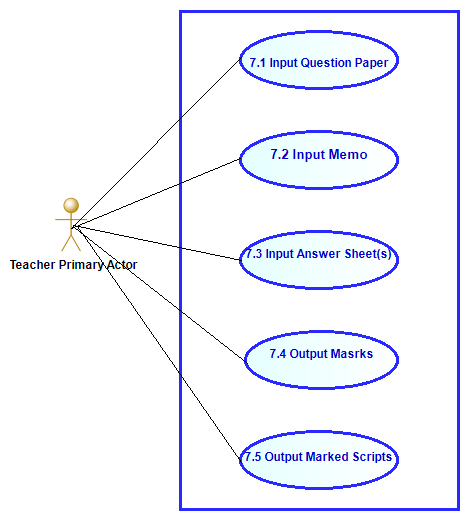
\includegraphics[scale=0.6]{Images/IO_Module/IOModuleUseCase}
			\caption{I/O Module Use Case}
		\end{figure}
		
		\subsubsection{Domain Model}
					\begin{figure}[h]
				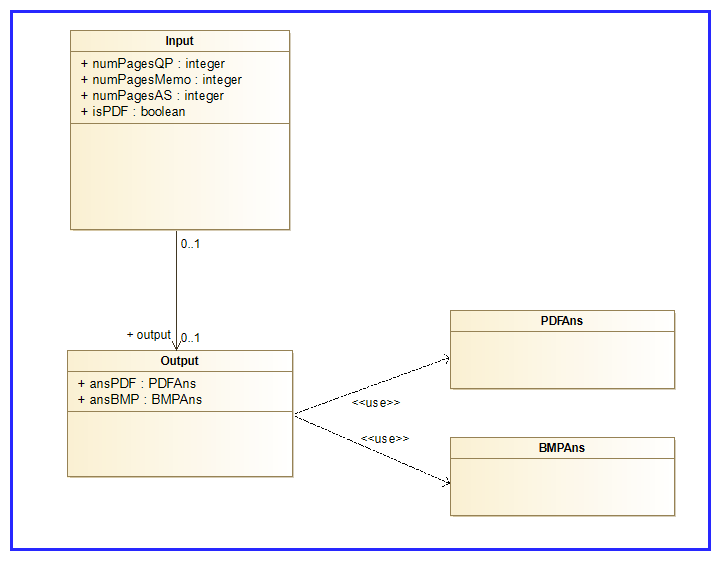
\includegraphics[scale=0.6]{Images/IO_Module/IOModuleDomainModel}
				\caption{I/O Module Domain Model}
			\end{figure}
			
		\subsubsection{Service Contracts}
					\begin{figure}[h]
				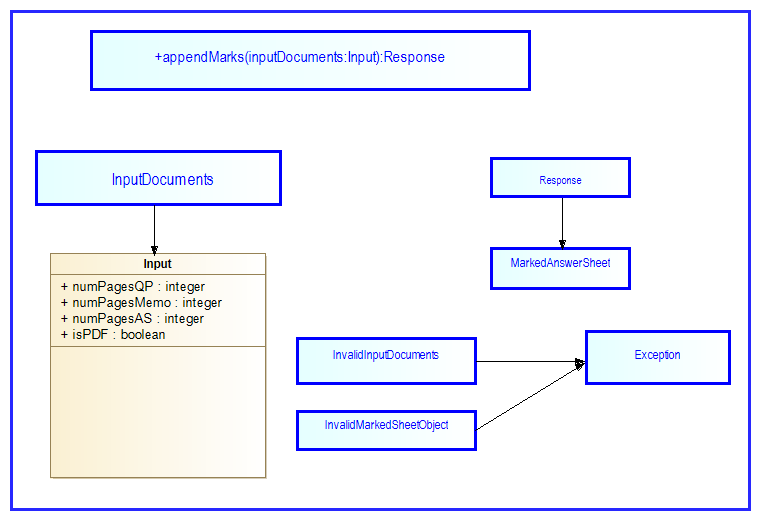
\includegraphics[scale=0.6]{Images/IO_Module/IOModuleServiceContracts}
				\caption{I/O Module Service Contracts}
			\end{figure}
			
		\subsubsection{Technologies}
					\begin{itemize}
				\item Img2Pdf - Converts an Image to PDF
				\item PIL(PILLOW) - Image processing
			\end{itemize}
		
\end{document}
